Quoting @chadloder@kolektiva.social:
\url{https://kolektiva.social/@chadloder/109779354899957742} \#retoot

\begin{figure}
\centering
\pandocbounded{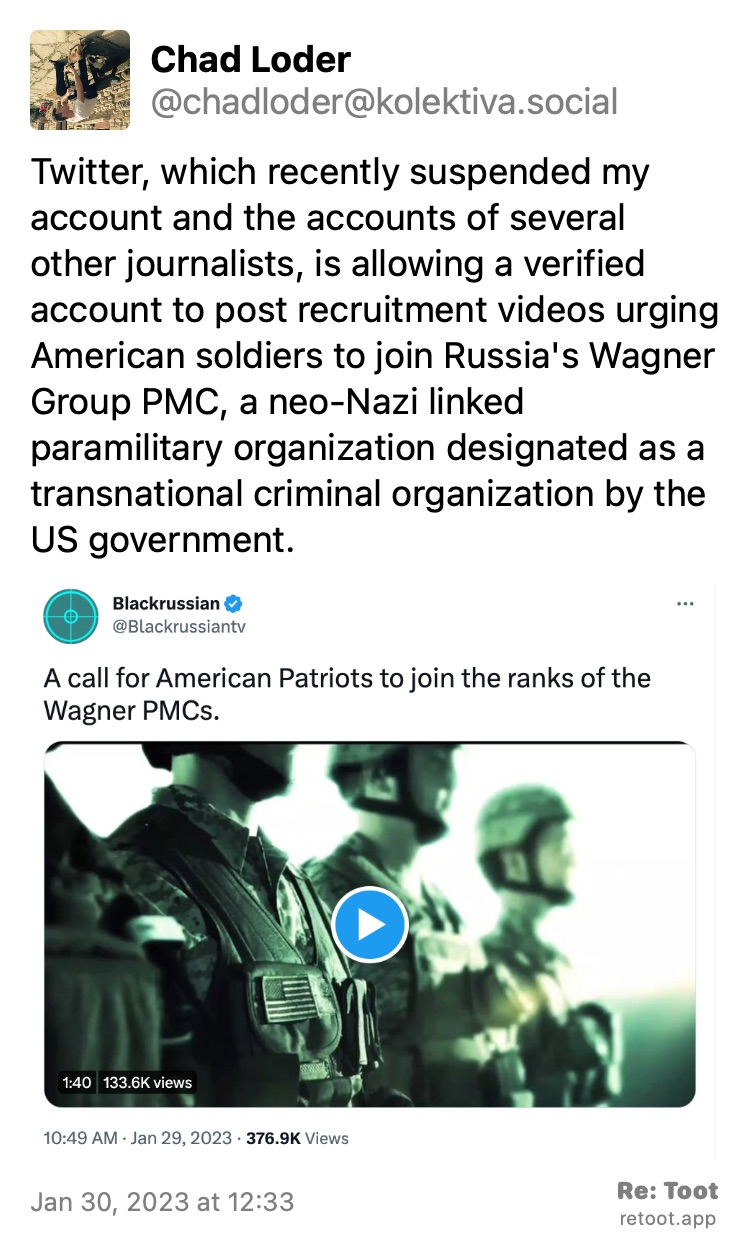
\includegraphics[keepaspectratio]{\%7B\%7Bsite.url\%7D\%7D/img/wagner-recruiting-in-usa.jpg}}
\caption{Post by Chad Loder. ``Twitter, which recently suspended my
account and the accounts of several other journalists, is allowing a
verified account to post recruitment videos urging American soldiers to
join Russia's Wagner Group PMC, a neo-Nazi linked paramilitary
organization designated as a transnational criminal organization by the
US government.'' The post contains an image with the following
description: ``Screenshot of a tweet by verified twitter account
@Blackrussiantv. The tweet reads''A call for American Patriots to join
the ranks of Wagner PMCs.'' The video thumbnail shows a green-tinted
shot of soldiers wearing American flag patches on their chest rigs''
Posted on Jan 30, 2023 at 12:33 at
https://kolektiva.social/@chadloder/10977935489995774}
\end{figure}

Laws in the United States are weird at times. Yes, the Wagner Group was
designated a ``transnational criminal organization'' under the
President's economic sanctions powers. Those same powers don't cut the
Wagner Group off from Twitter as they're seemingly technically just
posting information and not engaging in economic transactions where
money changes hands.

I know the Russian Federation is getting desperate. Recruiting dudes
from the USA who are most likely going to be of the MAGA persuasion is
simply a bad thing. Foreign adventures for MAGA adherents gives them
experience that becomes useful if we wind up in a rerun of the January
6th incident.

More madness will likely come this year, it seems.
